%%%%%%%% ICML 2022 EXAMPLE LATEX SUBMISSION FILE %%%%%%%%%%%%%%%%%

\documentclass[nohyperref]{article}

% Recommended, but optional, packages for figures and better typesetting:
\usepackage{microtype}
\usepackage{graphicx}
\usepackage{subfigure}
\usepackage{booktabs} % for professional tables

% hyperref makes hyperlinks in the resulting PDF.
% If your build breaks (sometimes temporarily if a hyperlink spans a page)
% please comment out the following usepackage line and replace
% \usepackage{icml2022} with \usepackage[nohyperref]{icml2022} above.
\usepackage{hyperref}


% Attempt to make hyperref and algorithmic work together better:
\newcommand{\theHalgorithm}{\arabic{algorithm}}

% Use the following line for the initial blind version submitted for review:
% \usepackage{icml2022}
\usepackage{pre-training}

% If accepted, instead use the following line for the camera-ready submission:
% \usepackage[accepted]{icml2022}

% For theorems and such
\usepackage{amsmath}
\usepackage{amssymb}
\usepackage{mathtools}
\usepackage{amsthm}

% if you use cleveref..
\usepackage[capitalize,noabbrev]{cleveref}

% custom
\usepackage{tabularx} % in the preamble
\usepackage{lipsum}
\usepackage{tabu}
\usepackage{booktabs}% for better rules in the table

%%%%%%%%%%%%%%%%%%%%%%%%%%%%%%%%
% THEOREMS
%%%%%%%%%%%%%%%%%%%%%%%%%%%%%%%%
\theoremstyle{plain}
\newtheorem{theorem}{Theorem}[section]
\newtheorem{proposition}[theorem]{Proposition}
\newtheorem{lemma}[theorem]{Lemma}
\newtheorem{corollary}[theorem]{Corollary}
\theoremstyle{definition}
\newtheorem{definition}[theorem]{Definition}
\newtheorem{assumption}[theorem]{Assumption}
\theoremstyle{remark}
\newtheorem{remark}[theorem]{Remark}

% Todonotes is useful during development; simply uncomment the next line
%    and comment out the line below the next line to turn off comments
%\usepackage[disable,textsize=tiny]{todonotes}
\usepackage[textsize=tiny]{todonotes}


% The \icmltitle you define below is probably too long as a header.
% Therefore, a short form for the running title is supplied here:
\icmltitlerunning{Submission and Formatting Instructions for ICML 2022}

\begin{document}

\twocolumn[
\icmltitle{Sample-Efficient finetuning by Interpreting skill as perspective}

% It is OKAY to include author information, even for blind
% submissions: the style file will automatically remove it for you
% unless you've provided the [accepted] option to the icml2022
% package.

% List of affiliations: The first argument should be a (short)
% identifier you will use later to specify author affiliations
% Academic affiliations should list Department, University, City, Region, Country
% Industry affiliations should list Company, City, Region, Country

% You can specify symbols, otherwise they are numbered in order.
% Ideally, you should not use this facility. Affiliations will be numbered
% in order of appearance and this is the preferred way.
\icmlsetsymbol{equal}{*}

\begin{icmlauthorlist}
\icmlauthor{Firstname1 Lastname1}{equal,yyy}
\icmlauthor{Firstname2 Lastname2}{equal,yyy,comp}
\icmlauthor{Firstname3 Lastname3}{comp}
\icmlauthor{Firstname4 Lastname4}{sch}
\icmlauthor{Firstname5 Lastname5}{yyy}
\icmlauthor{Firstname6 Lastname6}{sch,yyy,comp}
\icmlauthor{Firstname7 Lastname7}{comp}
%\icmlauthor{}{sch}
\icmlauthor{Firstname8 Lastname8}{sch}
\icmlauthor{Firstname8 Lastname8}{yyy,comp}
%\icmlauthor{}{sch}
%\icmlauthor{}{sch}
\end{icmlauthorlist}

\icmlaffiliation{yyy}{Department of XXX, University of YYY, Location, Country}
\icmlaffiliation{comp}{Company Name, Location, Country}
\icmlaffiliation{sch}{School of ZZZ, Institute of WWW, Location, Country}

\icmlcorrespondingauthor{Firstname1 Lastname1}{first1.last1@xxx.edu}
\icmlcorrespondingauthor{Firstname2 Lastname2}{first2.last2@www.uk}

% You may provide any keywords that you
% find helpful for describing your paper; these are used to populate
% the "keywords" metadata in the PDF but will not be shown in the document
\icmlkeywords{Machine Learning, ICML}

\vskip 0.3in
]

% this must go after the closing bracket ] following \twocolumn[ ...

% This command actually creates the footnote in the first column
% listing the affiliations and the copyright notice.
% The command takes one argument, which is text to display at the start of the footnote.
% The \icmlEqualContribution command is standard text for equal contribution.
% Remove it (just {}) if you do not need this facility.

%\printAffiliationsAndNotice{}  % leave blank if no need to mention equal contribution
\printAffiliationsAndNotice{\icmlEqualContribution} % otherwise use the standard text.

\begin{abstract}
Skill is an attempt to integrate pretrain-finetuning method in reinforcement learning.
During pretraining, the agent learns some useful and distinct policies without reward, and use this policy at finetuning to get fast and better performance than training from scratch.
However, there's few attempts to combine skills optimally at finetuning.
In this paper, we propose two skill combining methods which are sample-efficient and shows good performance.
First method is a state-agnostic super sample efficient method achieving higher reward than baseline methods adding only tens of parameters.
Second method is a state-aware skill combining method which is a slower-learner than first method but shows better performance at the end.
We improve second method's sample efficiency by using pretrained DIAYN module as a skill combining module.
Code is available at $https://github.com/some-private$.

\end{abstract}

%%%%%%%%% BODY TEXT
\section{introduction}
\label{submission}

Submission to ICML 2022 will be entirely electronic, via a web site
(not email). Information about the submission process and \LaTeX\ templates
are available on the conference web site at:
\begin{center}
\textbf{\texttt{http://icml.cc/}}
\end{center}

The guidelines below will be enforced for initial submissions and
camera-ready copies. Here is a brief summary:
\begin{itemize}
\item Submissions must be in PDF\@. 
\item \textbf{New to this year}: If your paper has appendices, submit the appendix together with the main body and the references \textbf{as a single file}. Reviewers will not look for appendices as a separate PDF file. So if you submit such an extra file, reviewers will very likely miss it.
\item Page limit: The main body of the paper has to be fitted to 8 pages, excluding references and appendices; the space for the latter two is not limited. For the final version of the paper, authors can add one extra page to the main body.
\item \textbf{Do not include author information or acknowledgements} in your
    initial submission.
\item Your paper should be in \textbf{10 point Times font}.
\item Make sure your PDF file only uses Type-1 fonts.
\item Place figure captions \emph{under} the figure (and omit titles from inside
    the graphic file itself). Place table captions \emph{over} the table.
\item References must include page numbers whenever possible and be as complete
    as possible. Place multiple citations in chronological order.
\item Do not alter the style template; in particular, do not compress the paper
    format by reducing the vertical spaces.
\item Keep your abstract brief and self-contained, one paragraph and roughly
    4--6 sentences. Gross violations will require correction at the
    camera-ready phase. The title should have content words capitalized.
\end{itemize}

\subsection{Submitting Papers}

\textbf{Paper Deadline:} The deadline for paper submission that is
advertised on the conference website is strict. If your full,
anonymized, submission does not reach us on time, it will not be
considered for publication. 

\textbf{Anonymous Submission:} ICML uses double-blind review: no identifying
author information may appear on the title page or in the paper
itself. \cref{author info} gives further details.

\textbf{Simultaneous Submission:} ICML will not accept any paper which,
at the time of submission, is under review for another conference or
has already been published. This policy also applies to papers that
overlap substantially in technical content with conference papers
under review or previously published. ICML submissions must not be
submitted to other conferences and journals during ICML's review
period.
%Authors may submit to ICML substantially different versions of journal papers
%that are currently under review by the journal, but not yet accepted
%at the time of submission.
Informal publications, such as technical
reports or papers in workshop proceedings which do not appear in
print, do not fall under these restrictions.

\medskip

Authors must provide their manuscripts in \textbf{PDF} format.
Furthermore, please make sure that files contain only embedded Type-1 fonts
(e.g.,~using the program \texttt{pdffonts} in linux or using
File/DocumentProperties/Fonts in Acrobat). Other fonts (like Type-3)
might come from graphics files imported into the document.

Authors using \textbf{Word} must convert their document to PDF\@. Most
of the latest versions of Word have the facility to do this
automatically. Submissions will not be accepted in Word format or any
format other than PDF\@. Really. We're not joking. Don't send Word.

Those who use \textbf{\LaTeX} should avoid including Type-3 fonts.
Those using \texttt{latex} and \texttt{dvips} may need the following
two commands:

{\footnotesize
\begin{verbatim}
dvips -Ppdf -tletter -G0 -o paper.ps paper.dvi
ps2pdf paper.ps
\end{verbatim}}
It is a zero following the ``-G'', which tells dvips to use
the config.pdf file. Newer \TeX\ distributions don't always need this
option.

Using \texttt{pdflatex} rather than \texttt{latex}, often gives better
results. This program avoids the Type-3 font problem, and supports more
advanced features in the \texttt{microtype} package.

\textbf{Graphics files} should be a reasonable size, and included from
an appropriate format. Use vector formats (.eps/.pdf) for plots,
lossless bitmap formats (.png) for raster graphics with sharp lines, and
jpeg for photo-like images.

The style file uses the \texttt{hyperref} package to make clickable
links in documents. If this causes problems for you, add
\texttt{nohyperref} as one of the options to the \texttt{icml2022}
usepackage statement.


\subsection{Submitting Final Camera-Ready Copy}

The final versions of papers accepted for publication should follow the
same format and naming convention as initial submissions, except that
author information (names and affiliations) should be given. See
\cref{final author} for formatting instructions.

The footnote, ``Preliminary work. Under review by the International
Conference on Machine Learning (ICML). Do not distribute.'' must be
modified to ``\textit{Proceedings of the
$\mathit{39}^{th}$ International Conference on Machine Learning},
Baltimore, Maryland, USA, PMLR 162, 2022.
Copyright 2022 by the author(s).''

For those using the \textbf{\LaTeX} style file, this change (and others) is
handled automatically by simply changing
$\mathtt{\backslash usepackage\{icml2022\}}$ to
$$\mathtt{\backslash usepackage[accepted]\{icml2022\}}$$
Authors using \textbf{Word} must edit the
footnote on the first page of the document themselves.
\section{Preliminaries and Related Work}
\textbf{Background.} We consider a Markov Decision Process (MDP) $\mathcal{M}=(\mathcal{S}, \mathcal{A}, p)$ without an external reward function for a typical unsupervised reinforcement learning. $\mathcal{S}$ is a state space, $\mathcal{A}$ is an action space, and $p(s'| s, a)$ is a dynamics. Given a skill $z$ sampling from a skill distribution $p(z)$, a policy $\pi(a | s, z)$ is learned in option framework.


\textbf{Skill discovery.} In unsupervised RL setting, \emph{skill discovery} is indicated to learn diverse behaviors with an intrinsic reward such as \emph{empowerment} \cite{salge2014empowerment}. This is formulated by maximizing mutual information between states and skills $\mathcal{I}(S; Z) = \mathcal{H}(S) - \mathcal{H}(S; Z) = \mathcal{H}(Z) - \mathcal{H}(Z; S)$, where $\mathcal{H}(\cdot)$ is the entropy in information theory. There are a number of previous methods to optimize the objective above. VIC \cite{gregor2016variational} and DIAYN \cite{eysenbach2018diversity} considers the final state and every state, respectively, in order to disciminate each skill. HIDIO \cite{zhang2021hierarchical} learns high level policy choosing skills in a hierarchical manner. APS \cite{liu2021aps} leverages successor feature to learn a diverse bahaviors. DADS \cite{sharma2019dynamics} focuses on the predictability of behaviors and learn dynamics. 

% SMM \cite{} and CIC \cite{} encourage agent to explore the state space while learning skills.

After the skill discovery phase, an agent should adapt to the task with learned skills. A simple but general method is to select one skill with initially highest reward for each task and further fine-tune this skill \cite{eysenbach2018diversity, laskin2022cic}. Some methods train an additional high level policy to choose skills to utilize more than just one skill for each task in a sequential way \cite{sharma2019dynamics}. For a specific purposed task such as a goal-reaching, there are zero shot skill adaptation methods \cite{sharma2019dynamics, choi2021variational}. We propose the general purposed but effective fine-tuning method for which a few additional parameters are needed to combine the skills.

TODO: Add DIAYN formulation (?)
% \input{contents/3_background}
\section{Proposed Method}
The main idea of our approach is to combine the learned skills to utilize for downstream tasks. 
We gain skills in the pretrain phase following DIAYN \cite{eysenbach2018diversity} framework which is used as a general skill discovery baseline.
In DIAYN, they only used one best performing skill at the finetuning phase.
However, it is often expensive to know which skill is best-performing and loses the possibility of gaining something from another independent skills. 
As a result, we propose several methods to combine skills $\pi(a|s,\psi(z))$.

We consider $[s,\psi(z)]$ to be a state representation from the view of skill $z$.
In other words, as many representations as the number of skills are created for one state.
We propose sample efficient but robust skill combining method.
% In this formulation, state representations are \emph{mixed} over the skills by the controller $p(z|s)$.
% As above, we may replace $p(z|s)$ to $p(z)$ for simplifying.
% In this case, we only need an additional weights on the simplex $w \in \Delta^k$ for $\mathbb{E}_{z \sim p(z)}[s,z] = f_{\psi}(\sum_i w_i[s,z_i])$. 

\subsection{State-agnostic perspective fusion}
We note that the skill $z$ is a $k$-dimensional discrete random variable sampled from the distribution $p(z)$.
This is same as to making a one-hot vector by filling in some positions with 0 vectors as many as $k$ predefined.
Then we hypothesize we could learn to use all skills if we fill all the places with 1's.
This is because skill implemented as a one-hot vector is just a policy that determines which of the neural net weights to activate.
Therefore, if all positions are filled with 1, all weights can be activated and more diverse representations can be obtained.
This is interpreting the same state from different perspectives through skill.
Vanilla DIAYN proposed to attain skill vector by sampling; $z \sim p(z|s)$
The example of $z=[1, 0, 0]$. Here we propose two ways to get these different persepctives. $\psi(z)$
The final policy will be $\pi(a|s,\psi(z))$. For $\psi$, we propose two ways.
First, we propose same-weight policy $\psi(z)=[\frac{1}{k}, \frac{1}{k}, \frac{1}{k}]$.

Second is simple parametric weight policy  $\psi(z)=[w_1, w_2, w_3]$.
The input state will be transformed into using these parameters. 
% $[s',z_i'] = \sum_{i}^{d}w_i [s,z_i]/d$
Then, the transformed state will be fed into policy network to generate an action.
% $a \sim g(\phi_i(s)), \text{where} \phi_i=f([s',z_i'])$
$a \sim \pi(s, [w_1,w_2,w_3])$





\subsection{State-aware perspective fusion}
In the above method, skill weight was determined without considering incoming state.
However, if the skill weight is changed adaptively according to the state, better performance may be achieved.
DIAYN module was a skill classifier in the pretraining phase, outputting which skill was in charge for the input state.
The final output of DIAYN is logit, which could be easily trasferred to probability when feeded in softmax layer.
We utilize this probability as a importance weight for skill. During the pretraining process, 
diayn $q_{\phi}(z|s)$ predicted skill through the state and we think this pretrain task help diayn module to learn combine skills  to incoming state.
Therefore, we propose to use DIAYN learned during pretraining as skill weight predictor.
$\pi(a|s,z)$ now transforms to equation \ref{eqn:daiyn as weight predictor}.

% We decompose a skill-conditioned policy to $\pi(a|s,z) = f_{\psi}(g_{\phi}(s, z))$ where $f_{\psi}$ is a linear classifier and $g_{\phi}$ is the rest.
% Then, we write a skill-agnostic policy as
\begin{equation}
\label{eqn:daiyn as weight predictor}
    % \tilde{\pi}(a|s) = f_{\psi}(\mathbb{E}_{z \sim p(z|s)}[g_{\phi}(s,z)])
    \pi(a|s,q_{\phi}(z|s))
\end{equation}


\subsection{Analyzation}
TODO: analyze a trajectory and the representations of each state



\section*{experiments}
Authors are kindly asked to make their submissions as accessible as possible for everyone including people with disabilities and sensory or neurological differences.
Tips of how to achieve this and what to pay attention to will be provided on the conference website \url{http://icml.cc/}.

\section*{Software and Data}

If a paper is accepted, we strongly encourage the publication of software and data with the
camera-ready version of the paper whenever appropriate. This can be
done by including a URL in the camera-ready copy. However, \textbf{do not}
include URLs that reveal your institution or identity in your
submission for review. Instead, provide an anonymous URL or upload
the material as ``Supplementary Material'' into the CMT reviewing
system. Note that reviewers are not required to look at this material
when writing their review.

\section{Conclusion}

In this paper, we propose a new fine-tuning method for skill discovery for combining learned skills efficiently.
By combining skills on the representation level rather than an action level,
it is possible to generalize the previous method and outperform other unsupervised RL methods in a sample efficiency manner.
We emphasize the importance of fine-tuning method for measuring the performance for a skill discovery method
and encourage the research direction for other skill mix method for future work.


% In this paper, we propose a method to enable faster and better learning by combining the skills learned in the pretrain phase.
% The interesting thing is that it is better to have a skill weight regardless of the state than to have a different skill weight for each state.
% Based on these results, we want to find a way to better utilize skill combinations such as attention in the future.



% \subsection{Attention}
% \begin{figure}[hb]
%   \vskip 0.2in
%   \begin{center}
%   \centerline{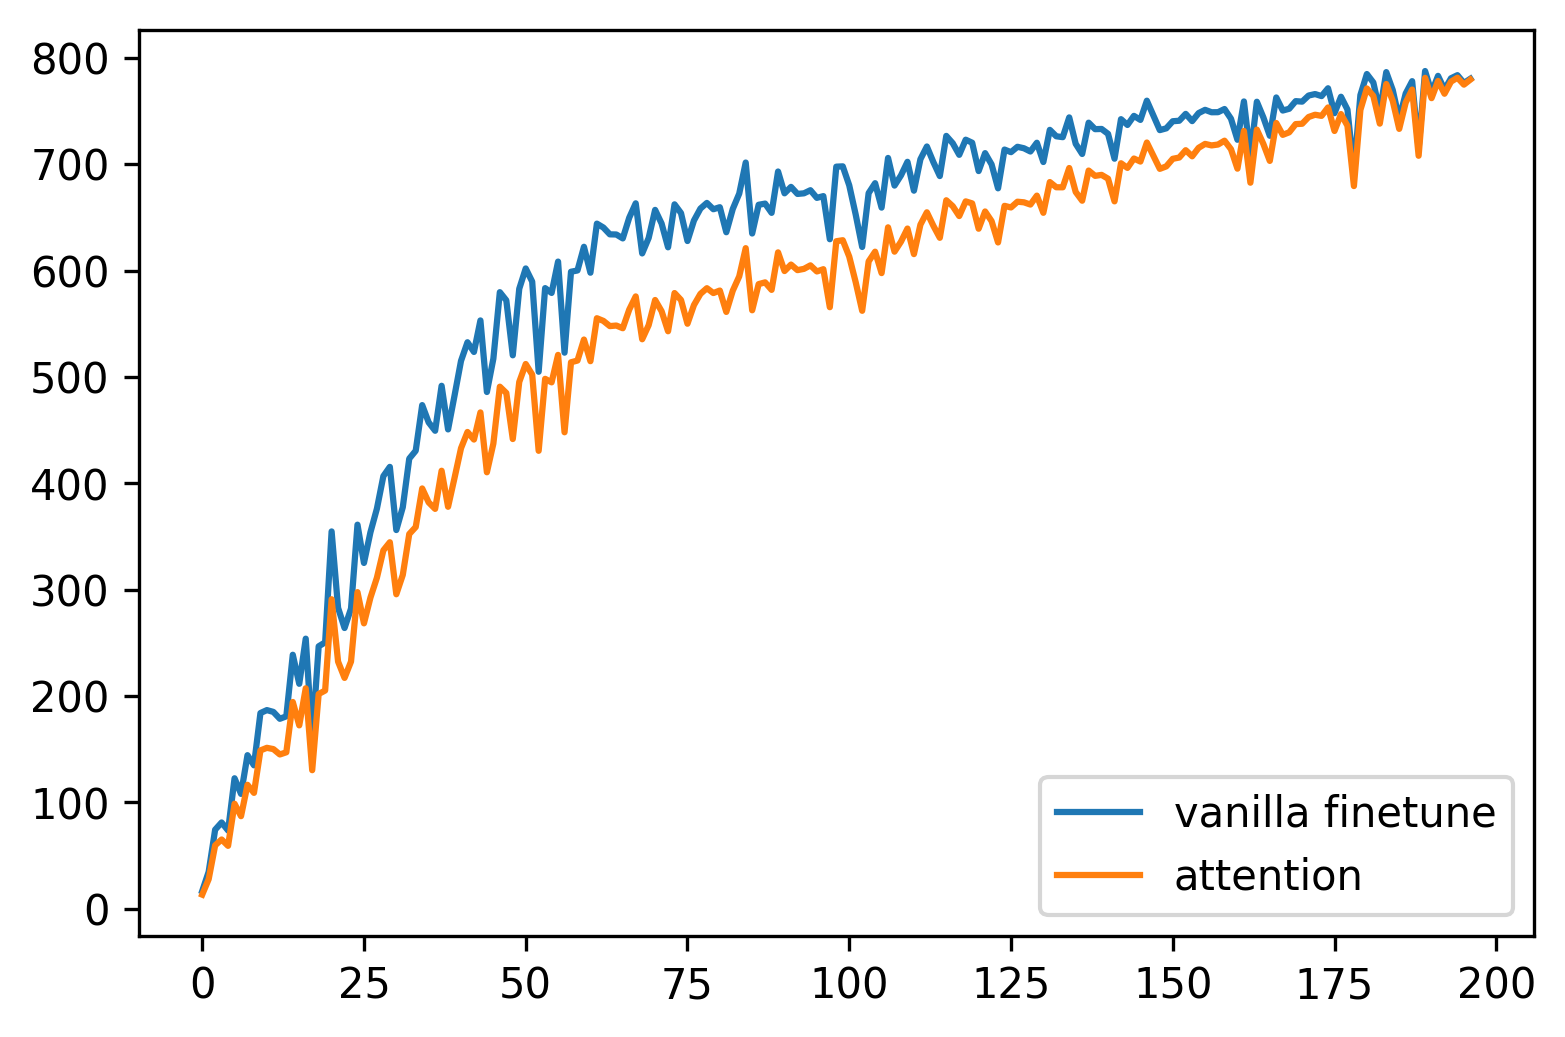
\includegraphics[width=\columnwidth]{Figures/attention_on_walker_run.png}}
%   \caption{This result was lost}
%   \label{attention-on-walker-run}
%   \end{center}
%   \vskip -0.2in
%   \end{figure}



% Camera-ready copies should have the title of the paper as running head
% on each page except the first one. The running title consists of a
% single line centered above a horizontal rule which is $1$~point thick.
% The running head should be centered, bold and in $9$~point type. The
% rule should be $10$~points above the main text. For those using the
% \textbf{\LaTeX} style file, the original title is automatically set as running
% head using the \texttt{fancyhdr} package which is included in the ICML
% 2022 style file package. In case that the original title exceeds the
% size restrictions, a shorter form can be supplied by using

% \verb|\icmltitlerunning{...}|

% just before $\mathtt{\backslash begin\{document\}}$.
% Authors using \textbf{Word} must edit the header of the document themselves.





% Acknowledgements should only appear in the accepted version.
% \section*{Acknowledgements}

% \textbf{Do not} include acknowledgements in the initial version of
% the paper submitted for blind review.

% If a paper is accepted, the final camera-ready version can (and
% probably should) include acknowledgements. In this case, please
% place such acknowledgements in an unnumbered section at the
% end of the paper. Typically, this will include thanks to reviewers
% who gave useful comments, to colleagues who contributed to the ideas,
% and to funding agencies and corporate sponsors that provided financial
% support.


% In the unusual situation where you want a paper to appear in the
% references without citing it in the main text, use \nocite
\nocite{langley00}

\bibliography{example_paper}
\bibliographystyle{icml2022}


%%%%%%%%%%%%%%%%%%%%%%%%%%%%%%%%%%%%%%%%%%%%%%%%%%%%%%%%%%%%%%%%%%%%%%%%%%%%%%%
%%%%%%%%%%%%%%%%%%%%%%%%%%%%%%%%%%%%%%%%%%%%%%%%%%%%%%%%%%%%%%%%%%%%%%%%%%%%%%%
% APPENDIX
%%%%%%%%%%%%%%%%%%%%%%%%%%%%%%%%%%%%%%%%%%%%%%%%%%%%%%%%%%%%%%%%%%%%%%%%%%%%%%%
%%%%%%%%%%%%%%%%%%%%%%%%%%%%%%%%%%%%%%%%%%%%%%%%%%%%%%%%%%%%%%%%%%%%%%%%%%%%%%%
\newpage
\appendix
\onecolumn
\section{You \emph{can} have an appendix here.}

%% TABLE %%%%%%%%%%%%%%%%%%%%%%%%%%%%%
\begin{table*}[t]
    \caption{Result of fine-tuning for $1 \times 10^5$ frames after pre-training for $2 \times 10^6$ frames.}
    \label{table:result_urlb}
    \vskip 0.15in
    \begin{center}
    \begin{small}
    \begin{sc}
    \begin{tabular}{lccccc}
    % \begin{tabular*}{\textwidth}{c @{\extracolsep{\fill}} ccccc}
    \toprule
    Domain & Task & Expert & Other best & Original DIAYN & Ours (same weight) \\
    \midrule
    Walker & Flip  & 799  & 515$\pm$17 &  381$\pm$17   & \textbf{658$\pm$51}\\
           & Run   & 796  & 439$\pm$34 &  242$\pm$11   & \textbf{537$\pm$22}\\
           & Stand & 984  & 923$\pm$9  &  860$\pm$26   & \textbf{936$\pm$11} \\
           & Walk  & 971  & 828$\pm$29 &  661$\pm$26   & \textbf{917$\pm$23}\\
    Quadruped & Jump  & 888  & 590$\pm$33  &  578$\pm$46  & \textbf{645$\pm$20} \\
           & Run   & 888     & 465$\pm$37  &  415$\pm$28  & \textbf{558$\pm$43} \\
           & Stand & 920     & \textbf{840$\pm$33}  &  706$\pm$48  & 719$\pm$158 \\
           & Walk  & 866     & 721$\pm$56  &  406$\pm$64  & \textbf{845$\pm$74}  \\
    Jaco & Reach bottom left   & 193 & 134$\pm$8 & 17$\pm$5   & \textbf{136$\pm$36}\\
           & Reach bottom right& 203 & \textbf{122$\pm$4} & 31$\pm$4   & 119$\pm$39\\
           & Reach top left    & 191 & 124$\pm$20 & 11$\pm$3   & \textbf{127$\pm$9}\\
           & Reach top right   & 223 & \textbf{140$\pm$7}  & 19$\pm$4   & 138$\pm$42\\
    \bottomrule
    \end{tabular}
    \end{sc}
    \end{small}
    \end{center}
    \vskip -0.1in
    \end{table*}
   %% TABLE %%%%%%%%%%%%%%%%%%%%%%%%%%%%%
%%%%%%%%%%%%%%%%%%%%%%%%%%%%%%%%%%%%%%%%%%%%%%%%%%%%%%%%%%%%%%%%%%%%%%%%%%%%%%%
%%%%%%%%%%%%%%%%%%%%%%%%%%%%%%%%%%%%%%%%%%%%%%%%%%%%%%%%%%%%%%%%%%%%%%%%%%%%%%%


\end{document}


% This document was modified from the file originally made available by
% Pat Langley and Andrea Danyluk for ICML-2K. This version was created
% by Iain Murray in 2018, and modified by Alexandre Bouchard in
% 2019 and 2021 and by Csaba Szepesvari, Gang Niu and Sivan Sabato in 2022. 
% Previous contributors include Dan Roy, Lise Getoor and Tobias
% Scheffer, which was slightly modified from the 2010 version by
% Thorsten Joachims & Johannes Fuernkranz, slightly modified from the
% 2009 version by Kiri Wagstaff and Sam Roweis's 2008 version, which is
% slightly modified from Prasad Tadepalli's 2007 version which is a
% lightly changed version of the previous year's version by Andrew
% Moore, which was in turn edited from those of Kristian Kersting and
% Codrina Lauth. Alex Smola contributed to the algorithmic style files.
